Tal como mencionamos en el desarrollo, la experimentación fue realizada para valores de $n= 4,6,8,10,12,16,32,64,128$. Entre 
ellos, fueron seleccionados los resultados más representativos y en donde creemos que se observa
mejor aquello que queremos mostrar.

\subsection{Variando el span}

Para este experimento, dado $n$, fijamos el valor de $h=n$, el valor de las cargas $c_{i}=1 \ \forall i$, y fuimos aumentando el
valor del \emph{span} en múltiplos de $n$, calculando en cada caso el valor de la máxima fuerza en módulo. Es decir, en primer lugar
$span=1*n$, luego $span=2*n$, \ldots.

\begin{figure}[!h]
	\begin{center}
		  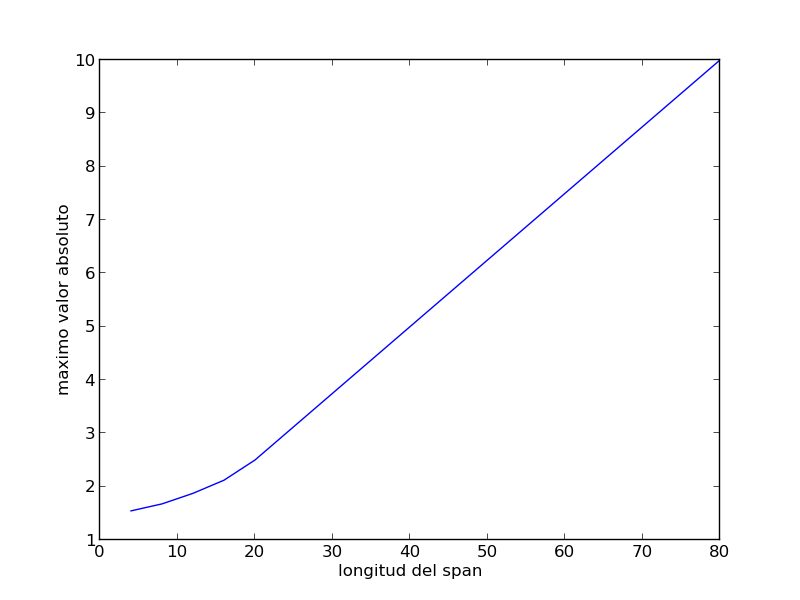
\includegraphics[scale=0.4]{Imagenes/variable_span/n_4}
		  \caption{Máxima fuerza en módulo en función de la longitud del span, para $n=4$}
		  \label{fig:contra1}
	\end{center}
\end{figure}
\FloatBarrier

\begin{figure}[!h]
	\begin{center}
		  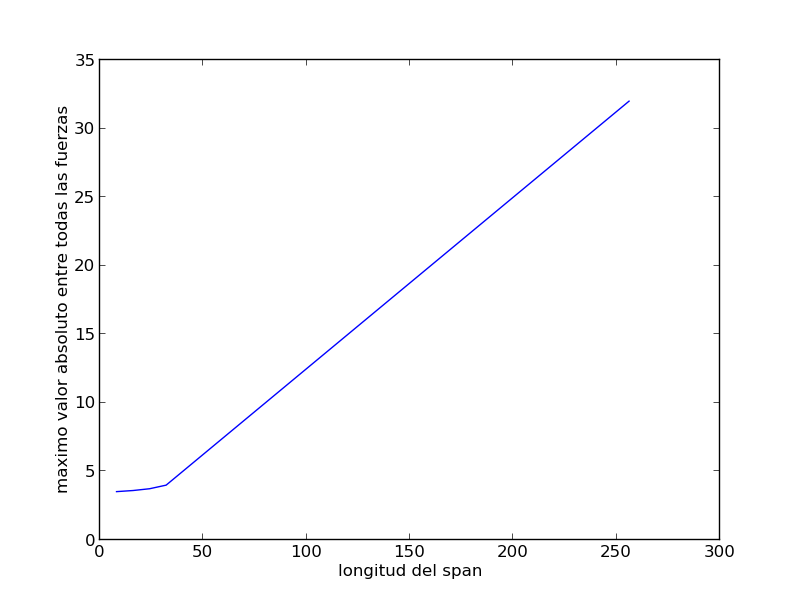
\includegraphics[scale=0.4]{Imagenes/variable_span/n_8}
		  \caption{Máxima fuerza en módulo en función de la longitud del span, para $n=8$}
		  \label{fig:contra1}
	\end{center}
\end{figure}
\FloatBarrier

\begin{figure}[!h]
	\begin{center}
		  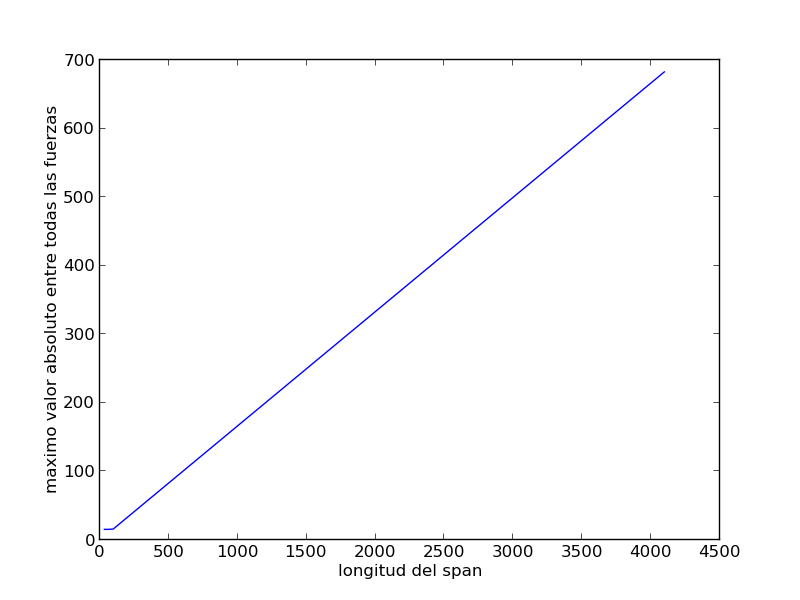
\includegraphics[scale=0.4]{Imagenes/variable_span/n_32}
		  \caption{Máxima fuerza en módulo en función de la longitud del span, para $n=32$}
		  \label{fig:contra1}
	\end{center}
\end{figure}
\FloatBarrier

Los resultados nos permiten corroborar nuestra primera hipótesis: El módulo de las fuerzas ejercidas sobre los links aumentan en función
del \emph{span}. Según lo que muestran los gráficos parecería ser que este aumento se da de forma directamente proporcional. Un hecho
importante que no estamos observando es que en los 3 experimentos, para cualquier valor de $n$, el link sobre el cual se ejerce 
la fuerza de módulo máximo es $2*n-1$. (Es algo razonable, teniendo en cuenta que el peso de las cargas está uniformemente 
distribuído).

~

\begin{figure}[!h]
	\begin{center}
		  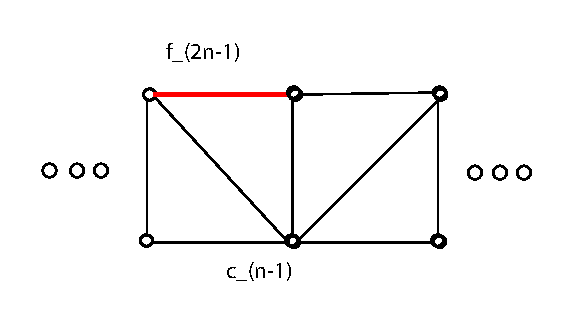
\includegraphics[scale=0.75]{Imagenes/im_12.pdf}
		  \caption{Fuerza $2*n-1$}
		  \label{fig:contra1}
	\end{center}
\end{figure}
\FloatBarrier

~

\subsection{Variando el valor de las cargas}

\subsubsection{Aumentando el peso de una única carga}

En primer lugar realizamos un experimento en donde únicamente variamos el valor de una de las cargas, manteniendo fijos el $span=n$
y $h=n$. En otras palabras, siendo $n$ la cantidad de secciones, generamos $\frac{n}{2}$ instancias distintas en donde el valor
de las cargas varía de la siguiente manera:

1) En la primera, peso de la carga aplicada sobre $c_{1}=100$ (primera junta inferior con carga)
. Peso de las cargas aplicadas sobre el resto de las juntas = 1.

2) En la segunda, peso de la carga aplicada sobre $c_{3}=100$ (segunda junta inferior con carga)
. Peso de las cargas aplicadas sobre el resto de las juntas = 1.

\ldots

n/2) En la $\frac{n}{2}$, peso de la carga aplicada sobre $c_{(n-1)}=100$. (junta inferior del medio con carga).
Peso de las cargas aplicadas sobre el resto de las juntas = 1.

~

A continuación se exhiben los resultados obtenidos para valores de $n=6,8,16$

\underline{Experimentación con $c_{1} = 100$}

\begin{center}
    \small{
    \begin{tabular}{| l | l | l | l | l | }
    \hline
    n & max\_fuerza($c_{1}=100$) & link más afectado & max\_fuerza($c_{1}=0$) & link más afectado\\ \hline 
    6 & 120.208 & 3 & 4 & 11 \\ \hline
    8 & 127.456 & 3 & 7.5 & 15 \\ \hline
    16 & 141.863 & 3 & 31.5 & 31 \\ \hline
    \end{tabular}
    }
\end{center}

~

\underline{Experimentación con $c_{3} = 100$}

\begin{center}
    \small{
    \begin{tabular}{| l | l | l | l | l | }
    \hline
    n & max\_fuerza($c_{3}=100$) & link más afectado & max\_fuerza($c_{3}=0$) & link más afectado\\ \hline 
    6 & 136 & 7 & 3.5 & 11 \\ \hline
    8 & 154.5 & 7 & 7 & 15 \\ \hline
    16 & 187.25 & 7 & 31 & 31 \\ \hline
    \end{tabular}
    }
\end{center}

~

En función de los valores obtenidos podemos observar 2 aspectos que corroboran nuestras hipótesis:

1) Cuando se aplica un peso mayor sobre una determinada junta $c_{i}$, la fuerza de mayor módulo es aquella que se
ejerce sobre el link $2*i+1$.

2) El módulo de las fuerzas sobre los links disminuye considerablemente cuando retiramos la carga más pesada (representado
por la tercera columna de las tablas). En esos casos, el link sobre el cual se ejerce la máxima fuerza vuelve a ser
$2*n-1$.

Incluimos un gráfico para esquematizar la idea planteada en el punto 1):

\begin{figure}[!h]
	\begin{center}
		  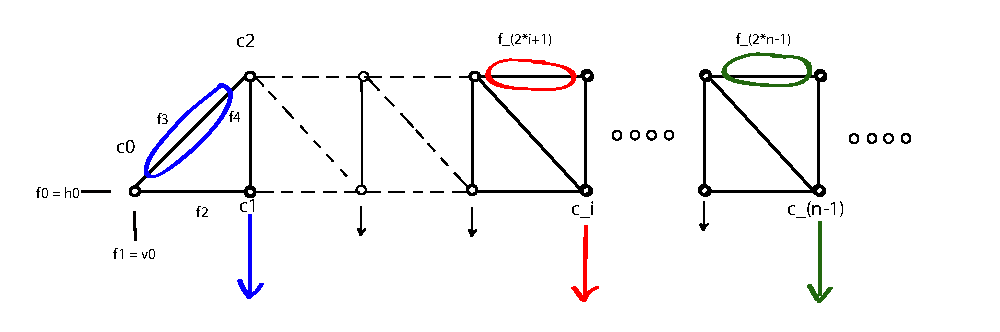
\includegraphics[keepaspectratio]{Imagenes/im_11.pdf}
		  \caption{Mayor carga aplicada sobre $c_{i} \Rightarrow$ fuerza de mayor módulo=$2*i+1$}
		  \label{fig:contra1}
	\end{center}
\end{figure}
\FloatBarrier

\subsubsection{Aumentando uniformemente el peso de todas las cargas}

En esta etapa de la experimentación aumentamos el peso de todas las cargas de igual manera. Para un determinado valor de $n$
fijamos $h=n$, $span=n$, y variamos el valor del peso de las cargas con valores entre 5 y 100 con saltos de 5 en 5. Los
resultados obtenidos fueron los siguientes:

\begin{figure}[!h]
	\begin{center}
		  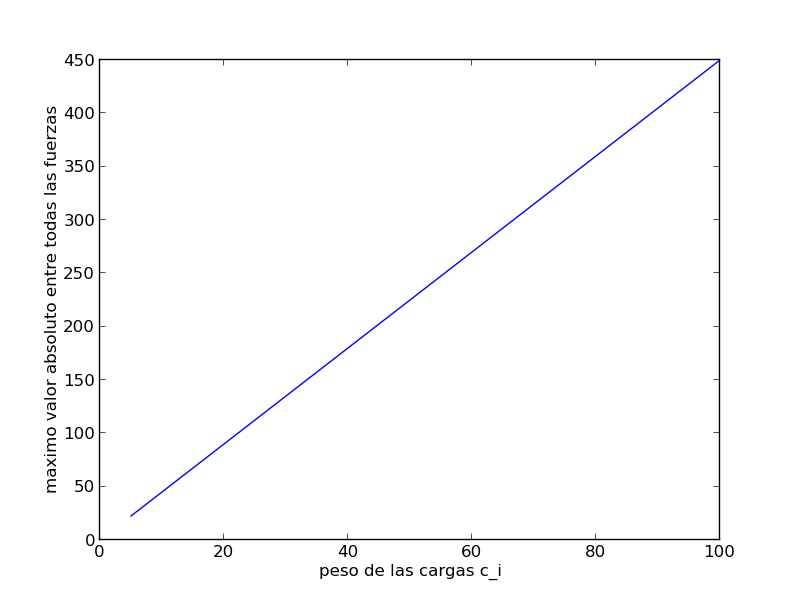
\includegraphics[scale=0.4]{Imagenes/variable_cis/equal_cis/equal_cis_n_6}
		  \caption{Máximo módulo de las fuerzas en función del peso de las cargas para $n=6$}
		  \label{fig:contra1}
	\end{center}
\end{figure}
\FloatBarrier

\begin{figure}[!h]
	\begin{center}
		  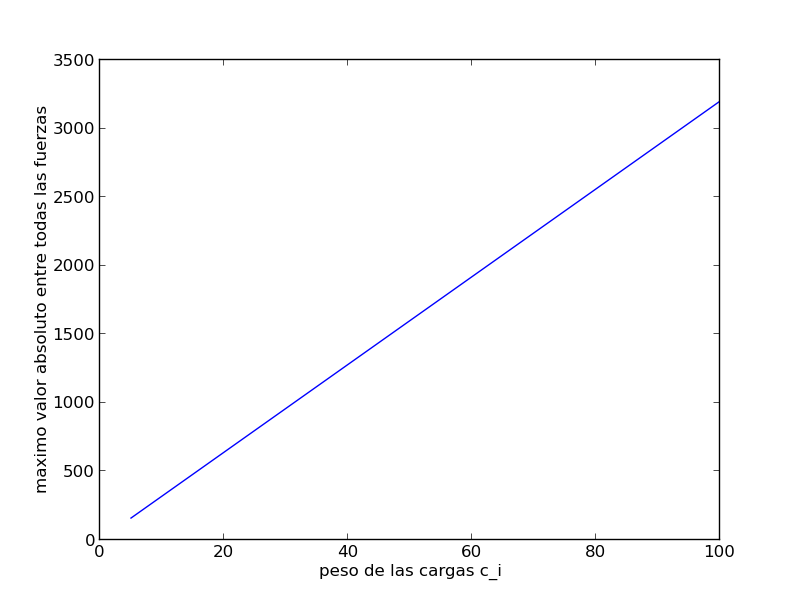
\includegraphics[scale=0.4]{Imagenes/variable_cis/equal_cis/equal_cis_n_16}
		  \caption{Máximo módulo de las fuerzas en función del peso de las cargas para $n=16$}
		  \label{fig:contra1}
	\end{center}
\end{figure}
\FloatBarrier

\begin{figure}[!h]
	\begin{center}
		  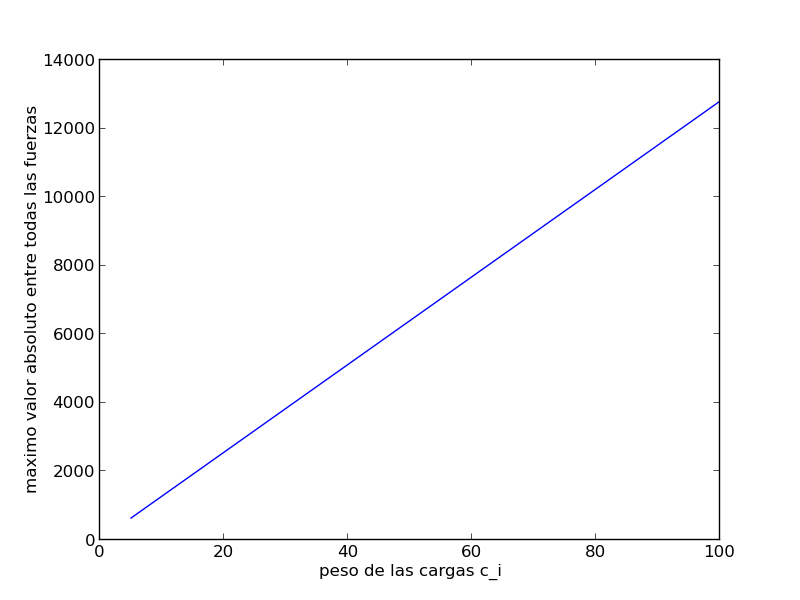
\includegraphics[scale=0.4]{Imagenes/variable_cis/equal_cis/equal_cis_n_32}
		  \caption{Máximo módulo de las fuerzas en función del peso de las cargas para $n=32$}
		  \label{fig:contra1}
	\end{center}
\end{figure}

Nuevamente, parecería ser el aumento del máximo módulo entre todas las fuerzas es directamente proporcional al peso de
todas las cargas. Observemos que comparando el experimento anterior y este para los mismos valores de $n$, el 
máximo módulo cuando se aumenta el peso de todas las cargas es mucho mayor que cuando se aumenta el peso de solo una de
ellas.

\subsubsection{Aumentando únicamente el peso de la carga del medio}

Las condiciones de este último experimento son muy similares a las del anterior: Para un determinado $n$,
$span=n$, $h=n$. Sin embargo, en este caso el peso de las cargas = 1 para todas menos para la central.
Vamos variando este último entre 5 y 100, con saltos de 5 en 5

\begin{figure}[!h]
	\begin{center}
		  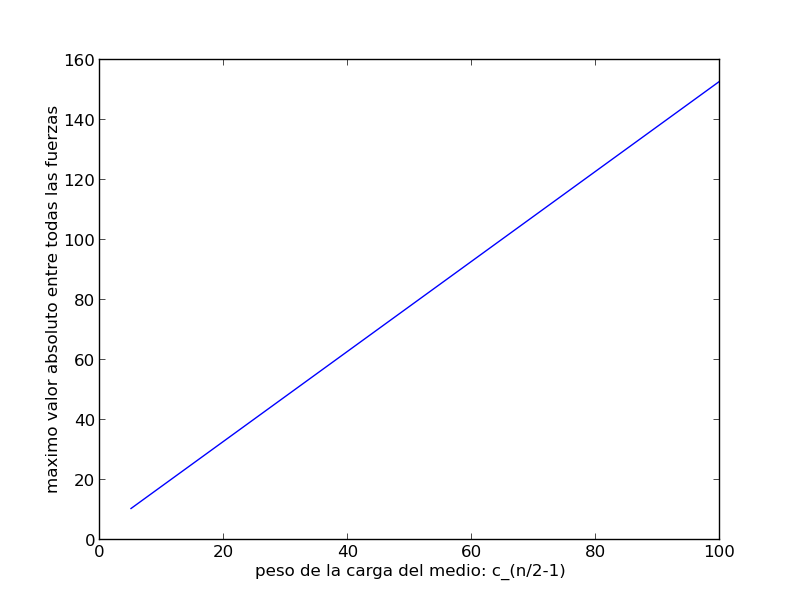
\includegraphics[scale=0.4]{Imagenes/variable_cis/just_middle_ci/just_middle_ci_n_6}
		  \caption{Máximo módulo de las fuerzas en función del peso de las carga del medio para $n=6$}
		  \label{fig:contra1}
	\end{center}
\end{figure}

\begin{figure}[!h]
	\begin{center}
		  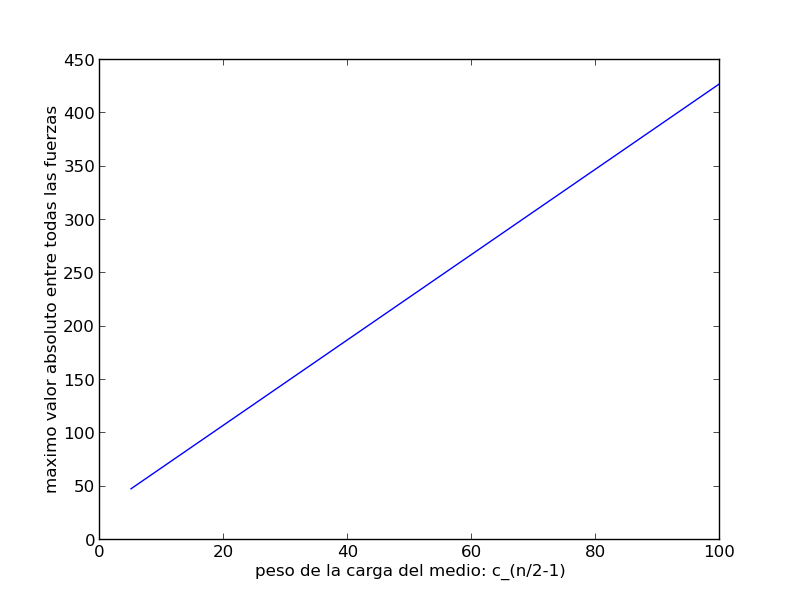
\includegraphics[scale=0.4]{Imagenes/variable_cis/just_middle_ci/just_middle_ci_n_16}
		  \caption{Máximo módulo de las fuerzas en función del peso de las carga del medio para $n=16$}
		  \label{fig:contra1}
	\end{center}
\end{figure}

\begin{figure}[!h]
	\begin{center}
		  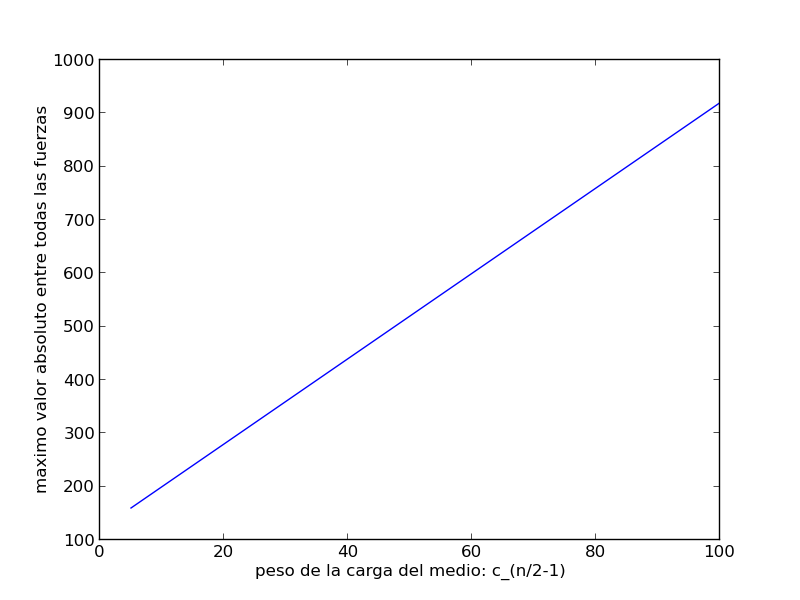
\includegraphics[scale=0.4]{Imagenes/variable_cis/just_middle_ci/just_middle_ci_n_32}
		  \caption{Máximo módulo de las fuerzas en función del peso de las carga del medio para $n=32$}
		  \label{fig:contra1}
	\end{center}
\end{figure}

Nuevamente observamos un aumento directamente proporcional entre ambas variables. Si bien no es posible verlo a partir de
los gráficos, también corroboramos la hipótesis planteada en el desarrollo respecto a la conservación de la
simetría de las fuerzas. Finalmente es necesario destacar que el aumento en el 
valor del máximo módulo para mismos valores de $n$ es mucho menor al del experimento anterior, en el que se aumentaba
el peso de todas las cargas.












